\documentclass{article} % For LaTeX2e
\usepackage{nips15submit_e,times}
\usepackage{hyperref}
\usepackage{url}
\usepackage{graphicx}
\usepackage{amsmath}
%\documentstyle[nips14submit_09,times,art10]{article} % For LaTeX 2.09
\newcommand\BibTeX{B{\sc ib}\TeX}

\title{LSTM for Sentiment Analysis on Twitter}

\author{
Trapit Bansal
\And
Kate Silverstein
\And
Jun Wang
}

%% \author{
%% David S.~Hippocampus\thanks{ Use footnote for providing further information
%% about author (webpage, alternative address)---\emph{not} for acknowledging
%% funding agencies.} \\
%% Department of Computer Science\\
%% Cranberry-Lemon University\\
%% Pittsburgh, PA 15213 \\
%% \texttt{hippo@cs.cranberry-lemon.edu} \\
%% \And
%% Coauthor \\
%% Affiliation \\
%% Address \\
%% \texttt{email} \\
%% \AND
%% Coauthor \\
%% Affiliation \\
%% Address \\
%% \texttt{email} \\
%% \And
%% Coauthor \\
%% Affiliation \\
%% Address \\
%% \texttt{email} \\
%% \And
%% Coauthor \\
%% Affiliation \\
%% Address \\
%% \texttt{email} \\
%% (if needed)\\
%% }


% The \author macro works with any number of authors. There are two commands
% used to separate the names and addresses of multiple authors: \And and \AND.
%
% Using \And between authors leaves it to \LaTeX{} to determine where to break
% the lines. Using \AND forces a linebreak at that point. So, if \LaTeX{}
% puts 3 of 4 authors names on the first line, and the last on the second
% line, try using \AND instead of \And before the third author name.

\newcommand{\fix}{\marginpar{FIX}}
\newcommand{\new}{\marginpar{NEW}}

\nipsfinalcopy % Uncomment for camera-ready version

\begin{document}


\maketitle

\begin{abstract}
abstract goes here
\end{abstract}

\section{Introduction}
% why analysis sentiment expecially twitter
In the last few years, microblogging has become a very popular communication tool in people's social life.
On microblogging platforms, such as Twitter\footnote{\url{https://twitter.com/}} and Facebook\footnote{\url{https://www.facebook.com/}}, a diverse range of people are attracted to post short sentences, images, and video links to share life issues and opinions.
This popularity results in enormous amount of information covering a wide range of topics on the brands, products, politics and social events. 
Such data is a valuable and efficient source for marketing and social studies. 
Sentiment analysis on microblogging has obtained special interest, because it determines the attitude of a user with respect to some topic or product and thus provides provide convincing information
For example, it may help manufacturing companies to know how people like their product (or service), what would people prefer.  

In this paper, we focus on using sentiment analysis on Twitter. 
Twitter is an extremely popular microblogging platform which allows people to post messages of up to 140 characters.
Because of the short nature of tweets, people often post twitter messages (called Tweets) frequently while attending events like product launches, movie premiers, music concerts or just to express their opinion on a trending or current topic.
As such, they can be a valuable source of public opinion or feedback \cite{o2010tweets, bollen2011twitter, bollen2009modeling}.
Realizing this importance, analyzing sentiment of Tweets has been a recurring task in the SemEval \footnote{\url{http://alt.qcri.org/semeval2016/task4/}} competitions.

%We restrict our interest on Twitter for the following reasons: 
%People are posting on various topics on Twitter, thus it is a valuable source of data; Twitter is one of the most popular microblogging platform and the number of messages are growing everyday. The collected corpus can be arbitrary large. Users of Twitter have various background and have different language conventions. It is possible to collect tweets of wide diversity in both topics and language models.

Although there exist plenty of work on text classification, some unique characteristics of tweets present special challenges for sentiment analysis:
1. Tweets are short in length. There is a limitation of $140$ words for each tweet; 2. The language used in tweets is very informal with misspelling, creative spelling,  new words, slangs, and URLs; 3. Emotions and hashtags are frequently used.

% what we did
In this paper, we propose a bi-directional Long Short-Term Memory (LSTM) method for sentiment analysis. We tried both word-level and character-level features on the bi-directional LSTM model and compare the results with Dynamic Convolutional Neural Network (DCNN) \cite{kalchbrenner2014convolutional}.
We show that the accuracy of sentiment analysis ... (Please revise this part.)

We train our model on $1.6$ M distantly-supervised tweets collected by Go et. al. \cite{go2009twitter}, and evaluate the results on SemEval-2016 Task 4\footnote{\url{http://alt.qcri.org/semeval2016/task4/}}. Currently we focus on polarity classification, and plan to apply our model on 5-point scale classification in the future. 

% the structure of the paper
In the remaining of this paper, we first introduce the related work, the dataset, and the evaluation methodology. We then describe the model we proposed. Finally, we discuss the experiment results and point out possible directions for future research. (Please revise this part.)

\section{Related Work}
Twitter sentiment analysis is increasingly drawing attention of researchers in recent years. 
Given the length limitations on tweets, sentiment analysis of tweets is often considered similar to sentence-level sentiment analysis \cite{kouloumpis2011twitter}.
However, phrase and sentence level approaches can hardly define the sentiment of some specific topics. Considering opinions adhering on different topics, Wang et. al. \cite{wang2011topic} proposed a hashtag-level sentiment classification method  to generate the overall sentiment polarity for a given hashtag.
Recently, following the work of \cite{mikolov2013efficient} some researchers used neural network to implement sentiment classification. 
For example, Kim \cite{kim2014convolutional} adopted convolutional neural networks to learn sentiment-bearing sentence vectors, Mikolov et al. \cite{mikolov2013distributed} proposed Paragraph vector which outperformed bag-of-words model for sentiment analysis, and Tang et. al. \cite{tang2014learning} used ConvNets to learn sentiment specific word embedding (SSWE), which encodes sentiment information in the continuous
representation of words.
Furthermore, Kalchbrenner \cite{kalchbrenner2014convolutional} proposed a Dynamic Convolutional Neural Network (DCNN) which uses dynamic k-max pooling, a global pooling operation over linear sequences.
Instead of directly applying ConvNets to embeddings of words, \cite{zhang2015character} applies the network only on characters. They showed that the deep ConvNets does not require knowledge of words and thus can work for different languages.
LSTM \cite{hochreiter1997long} is another state-of-the-art semantic composition models for sentiment classification \cite{li2015tree}. Similar to DCNN, it also learns fixed-length vectors for sentences of varying length, captures words order in a sentence and does not depend on external dependency or constituency parse results.

\subsection{Dynamic Convolutional Neural Networks (DCNN)}
We briefly review the architecture of DCNN \cite{kalchbrenner2014convolutional} which has shown state of the art performance for sentiment classification on Twitter. The winning entry for SemEval15 \cite{severynunitn} task on Twitter sentiment classification also used DCNN. Figure \ref{fig:dcnn} summarizes the architecture.

When used for sentiment classification on Twitter, the input to the DCNN is a matrix of word embeddings for each word in the tweet. For example, if the tweet consists of $s$ words then the input to the DCCNN is:
\begin{flalign*}
	S = 
	\begin{bmatrix}
	| & | & \ldots & | \\
	w_1 & w_2 & \ldots & w_s \\
	| & | & \ldots & | \\
	\end{bmatrix}_{k\times s}
\end{flalign*}
where each $w_i \in R^k$ is a $k$-dimensional dense word embedding \cite{mikolov2013distributed}.
The architecture consists of multiple layers of convolutions and max-pooling on top of the input matrix, followed a fully connected layer which is input to a softmax. The convolutions are of type \emph{wide-convolutions} of one-dimension. For example, for the input matrix $S \in R^{k\times s}$, a wide-convolution filter operating on $S$ will consist of convolution weights $m\in R^{k\times c}$ and will result in a matrix having dimension $k \times (s+c-1)$. Note here $c$ is the convolution filter width, which is a hyperparameter.
The max-pooling operations presented in \cite{kalchbrenner2014convolutional} are different from the regular max-pooling. They present {\it dynamic $k$-max pooling}. $k$-max pooling takes the top $k$ maximum activations as opposed to just the maximum activation and the value of $k$ is selected dynamically based on the following formula: $k_l = \max \left( k_{top}, 	\lceil \frac{L-l}{L} s\rceil \right)$, where $l$ is number of current convolution layer, $L$ is total number of convolutions and $k_{top}$ is a fixed hyperparameter. 
Note that while \cite{kalchbrenner2014convolutional} used multiple layers of convolutions and max-pooling, subsequent work found that using a single layer of convolution and max-pooling gives similar results \cite{kim2014convolutional} \cite{severynunitn}.

\begin{figure}
	\centering
	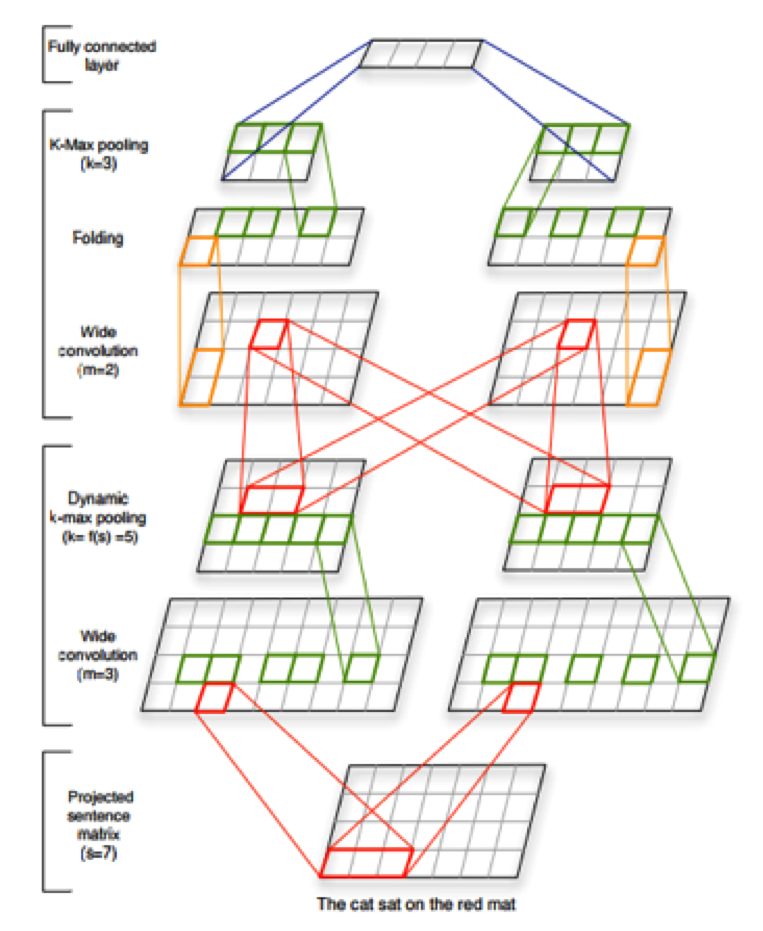
\includegraphics[height=4in, width=0.8\textwidth]{figs/DCNN.png}
	\caption{Dynamic Convulational Neural Network of \cite{kalchbrenner2014convolutional} (Source: \cite{kalchbrenner2014convolutional})}
	\label{fig:dcnn}
\end{figure}

\subsection{Recurrent Neural Networks with Long Short Term Memory (LSTM)}
Recurrent Neural Networks (RNNs) are a class of artificial neural networks used for modeling sequences.
RNNs are highly flexible in their use of context information as they can learn what part of the input sequence to store to memory and what parts to ignore. They also allow modeling of various regimes of sequence modeling as shown in Figure \ref{fig:rnn}. Please refer to \cite{graves2012supervised} for a comprehensive review of sequence modeling using RNN.

\begin{figure}
	\centering
	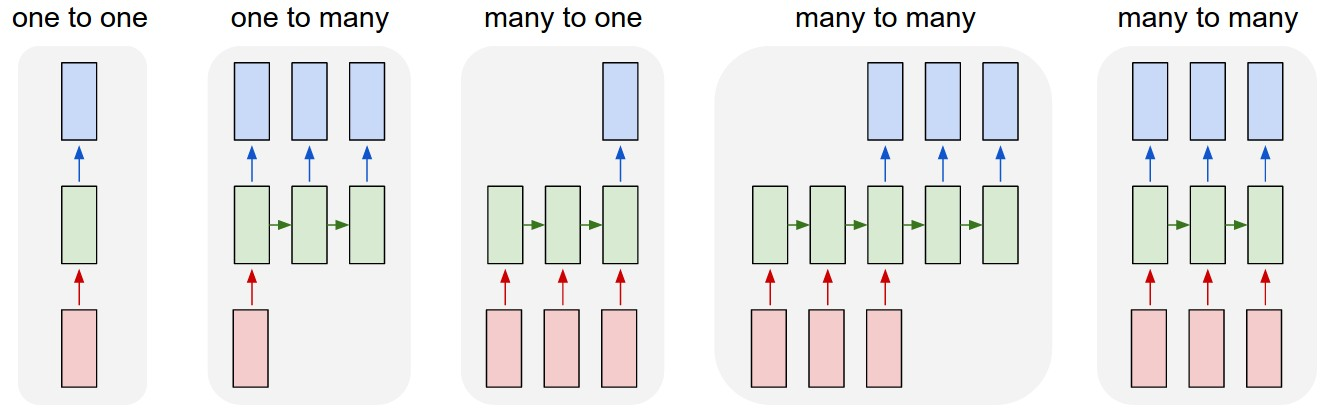
\includegraphics[width=\textwidth]{figs/rnn.jpeg}
	\caption{RNNs allow modeling of multiple types of input and output sequences (Source: \cite{karpathy-rnn})}
	\label{fig:rnn}
\end{figure}

One of the short comings of RNN is that it is very difficult to store information over long sequences because of problems due to vanishing and exploding gradients as explained in \cite{hochreiter2001gradient}.
{\it Long Short-Term Memory (LSTM)} \cite{hochreiter1997long} are designed to remedy this and store information over larger input sequences.
They achieve this using special ``memory cell'' units. 
Figure \ref{fig:lstm} shows the architecture of this cell which consists of an input gate, a forget gate, an output gate and a recurring cell state. 
Refer to \cite{colah} for a gentle introduction to LSTM and to \cite{graves2012supervised} for a more comprehensive review and applications.

\begin{figure}
	\centering
	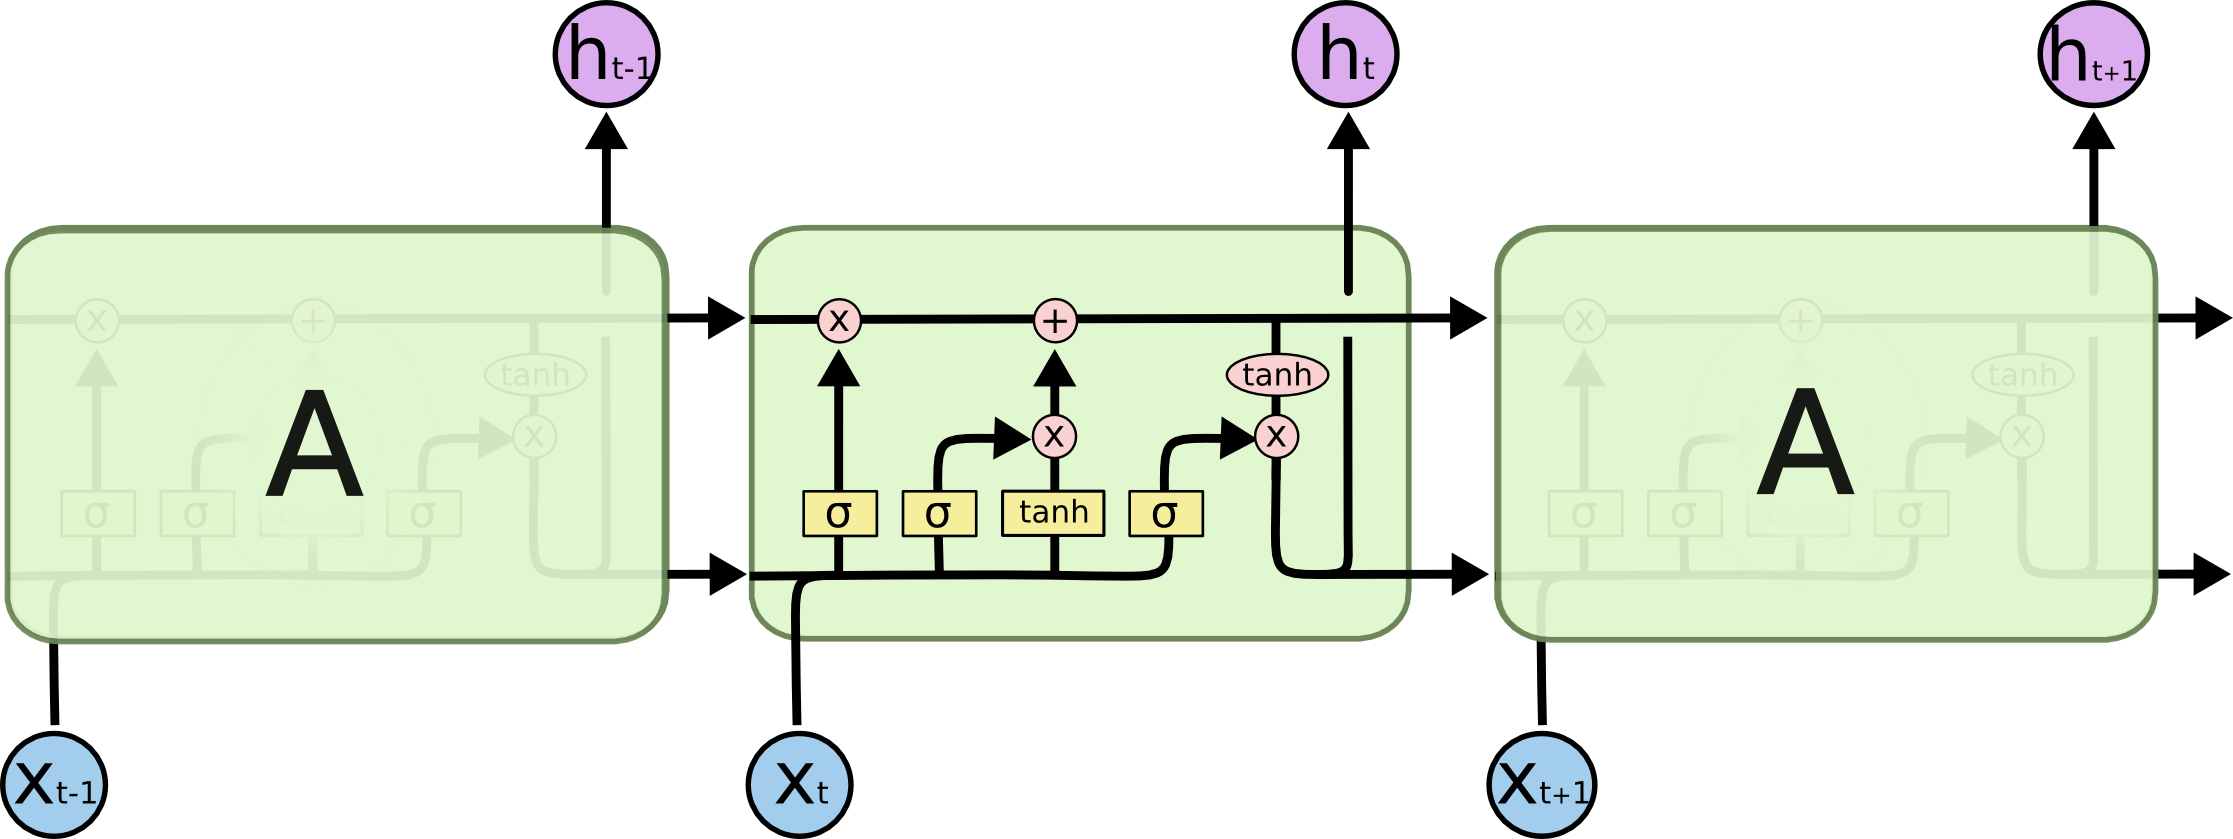
\includegraphics[width=\textwidth]{figs/LSTM.png}
	\caption{The repeating module of LSTM. $x_t$ is the input as time $t$ and $h_t$ is the output from the LSTM output gate at time $t$. The top horizontal line corresponds to the cell state and the bottom line corresponds to the hidden state (both of which are recurring states).
	(Source: \cite{colah})}
	\label{fig:lstm}
\end{figure}


\section{Twitter Sentiment Analysis using LSTM}


\section{Experiments}
See Table ~\ref{sample-table} for awesome results

\begin{table}[h]
\caption{Sample table title}
\label{sample-table}
\begin{center}
\begin{tabular}{ll}
\multicolumn{1}{c}{\bf PART}  &\multicolumn{1}{c}{\bf DESCRIPTION}
\\ \hline \\
Dendrite         &Input terminal \\
Axon             &Output terminal \\
Soma             &Cell body (contains cell nucleus) \\
\end{tabular}
\end{center}
\end{table}

This is a figure:

\begin{figure}[h]
\begin{center}
%\framebox[4.0in]{$\;$}
\fbox{\rule[-.5cm]{0cm}{4cm} \rule[-.5cm]{4cm}{0cm}}
\end{center}
\caption{Sample figure caption.}
\end{figure}

\section{Conclusion}


\subsubsection*{Acknowledgments}



\subsubsection*{References}

\bibliography{paper}
\bibliographystyle{plain}
%% References follow the acknowledgments. Use unnumbered third level heading for
%% the references. Any choice of citation style is acceptable as long as you are
%% consistent. It is permissible to reduce the font size to `small' (9-point) 
%% when listing the references. {\bf Remember that this year you can use
%% a ninth page as long as it contains \emph{only} cited references.}

%% \small{
%% [1] Alexander, J.A. \& Mozer, M.C. (1995) Template-based algorithms
%% for connectionist rule extraction. In G. Tesauro, D. S. Touretzky
%% and T.K. Leen (eds.), {\it Advances in Neural Information Processing
%% Systems 7}, pp. 609-616. Cambridge, MA: MIT Press.

%% [2] Bower, J.M. \& Beeman, D. (1995) {\it The Book of GENESIS: Exploring
%% Realistic Neural Models with the GEneral NEural SImulation System.}
%% New York: TELOS/Springer-Verlag.

%% [3] Hasselmo, M.E., Schnell, E. \& Barkai, E. (1995) Dynamics of learning
%% and recall at excitatory recurrent synapses and cholinergic modulation
%% in rat hippocampal region CA3. {\it Journal of Neuroscience}
%% {\bf 15}(7):5249-5262.
%% }

\end{document}
